\documentclass{book}
\usepackage[utf8]{inputenc}
\usepackage[T1]{fontenc}
\usepackage[dutch]{babel}
\usepackage{amsmath, amssymb}
\usepackage{tikz}
\usepackage{pgfplots}
\usepackage{epigraph}
\usepackage{hyperref}
\pgfplotsset{compat=1.17} % Zorgt voor compatibiliteit met recente pgfplots

\begin{document}
	\title{De wiskunde van Elvis Presley}
	\author{Jeroen Vermeulen}
	\maketitle
	
	
	\begin{abstract}
		In mijn leven zijn er drie constante: wiskunde, fysica en Elvis Presley. 
		Deze drie domeinen lijken op het eerste gezicht weinig gemeenschappelijk te hebben, maar in mijn 
		persoonlijke wereld vormen ze een samenhangend geheel van logica, schoonheid en fascinatie. Dit 
		document is het resultaat van een lang gekoesterde hobby: de vraag wat er gebeurt wanneer we het 
		fenomeen Elvis Presley niet benaderen vanuit muziekgeschiedenis of culturele analyse, maar vanuit 
		de bril van de wiskunde.
		
		In dit werk onderzoek ik verschillende fases van Elvis' carri\`ere met behulp van concepten uit de 
		exponenti\"ele groei, goniometrie, analyse, statistiek, waarschijnlijkheidstheorie en grafentheorie. 
		Door zijn artistieke evolutie te modelleren als functies, grafen, cycli en stochasticiteit, ontstaat 
		een onverwacht maar rijk beeld van een icoon dat zowel menselijk als structureel uniek was.
		
		Dit document is niet geschreven als academische verhandeling, maar als een persoonlijke en creatieve 
		exploratie van twee passies die mijn leven vormgeven. Wat volgt, is een poging om de wiskundige 
		structuren achter de energie, beweging, keuzes en evolutie van Elvis Presley zichtbaar te maken. 
		Voor mij was dit een intellectueel spel, een eerbetoon en een analytische ontdekkingsreis in één.
	\end{abstract}
	
	
	% ==========================
	% HOOFDSTUK 1
	% ==========================
	\chapter{De Exponenti\"ele Doorbraak (1954--1956)}
	\label{chap:exponentieel}
	
	\epigraph{Omnia apud et mathematica fiunt.}{Ren\'e Descartes}
	
	De carri\`ere van Elvis Presley in de periode 1954 tot 1956 is een schoolvoorbeeld van
	exponenti\"ele groei -- niet in een laboratorium, maar in de wereld van cultuur, muziek en roem.
	Wat begint als een lokale storm in Memphis, ontpopt zich binnen enkele jaren tot een wereldwijde
	orkaan van aandacht, bewondering en soms controverse. In dit hoofdstuk benaderen we deze periode
	niet louter als muziekgeschiedenis, maar als een casus van exponenti\"ele groei: een fenomeen dat
	in de wiskunde even vertrouwd is als in de natuur, fysica en economie.
	
	De observatie is eenvoudig: er zijn momenten in de geschiedenis waarop veranderingen niet
	geleidelijk verlopen, maar razendsnel accelereren. Een kleine verstoring, een nieuw idee of een
	ontluikend talent kan, onder de juiste omstandigheden, transformeren in een kettingreactie.
	Elvis Presley belichaamt in deze jaren precies zo'n kettingreactie. De combinaties van radio,
	televisie, platenverkoop en live-optredens werken als vermenigvuldigers in een
	exponentieel proces.
	
	Als wiskundige of fysicus is het dan haast onvermijdelijk om dit niet alleen als
	cultureel fenomeen te bekijken, maar ook als een dynamisch systeem. We kunnen de ``omvang van de roem''
	van Elvis modelleren als een functie van de tijd, en onderzoeken hoe snel die roem groeit, welke factoren
	als parameters kunnen worden ge\"interpreteerd, en of er aanwijzingen zijn voor verzadiging, limieten of
	zelfs instabiliteit.
	
	Om dit concreet te maken, introduceren we een eenvoudig model gebaseerd op de
	klassieke differentiaalvergelijking voor ongeremde groei. Laten we $N(t)$ defini\"eren als een maat voor de
	roem van Elvis op tijdstip $t$, waarbij $t$ wordt uitgedrukt in jaren sinds 1954. We zouden kunnen denken
	aan een genormaliseerde schaal waarin $N(t)$ bijvoorbeeld een combinatie is van platenverkoop, radio-airplay,
	televisieoptredens en concertbezoek. Hoewel de exacte definitie van $N(t)$ in de praktijk complex is, volstaat
	het voor ons doel om $N(t)$ te zien als een abstracte, maar groeiende grootheid.
	
	\section{Exponenti\"ele groei als model voor roem}
	
	Een klassiek model voor groei zonder remming is gegeven door de differentiaalvergelijking
	\[
	\frac{dN}{dt} = k N(t),
	\]
	waarbij $k > 0$ een constante is die de groeisnelheid bepaalt. De oplossing van deze vergelijking is
	bekend:
	\[
	N(t) = N_0 e^{kt},
	\]
	waarbij $N_0 = N(0)$ de beginwaarde is, in ons geval de roem of naamsbekendheid van Elvis in 1954, toen hij
	net zijn eerste opnames maakte bij Sun Records.
	
	Hoewel dit model idealiseert en geen rekening houdt met verzadiging of externe beperkingen, is het bijzonder
	geschikt om de vroege fase van zijn carri\`ere te beschrijven, waarin elk nieuw optreden leidde tot een disproportionele
	toename van aandacht. Radiostations pikten zijn muziek op, jonge fans reageerden heviger dan verwacht, en mediaorganen
	vergrootten die reacties verder uit. Dit werkt als een positieve terugkoppeling: hoe groter $N(t)$ wordt, hoe groter
	\(\frac{dN}{dt}\), de snelheid van verandering.
	
	In meer fysische termen: we hebben te maken met een proces waarin de ``veldsterkte'' van de roem toeneemt met de
	bron zelf. Hoe meer mensen Elvis kennen, hoe sneller nieuwe mensen hem leren kennen. Dit effect is kenmerkend voor
	exponenti\"ele systemen en vormt een belangrijk contrast met lineaire groei, waarin elke tijdseenheid een gelijke bijdrage
	levert.
	
	\section{Een eenvoudig model voor de doorbraakjaren}
	
	Laten we, ter illustratie, een hypothetisch maar representatief model opstellen voor de periode 1954--1956. Stel dat
	Elvis in 1954 een beginwaarde heeft van
	\[
	N_0 = 10,
	\]
	op een arbitraire schaal voor roem. We nemen aan dat zijn roem groeit met een continue groeifactor $k = 0.5$ per jaar.
	Onze functie wordt dan:
	\[
	N(t) = 10 e^{0.5 t}.
	\]
	
	Voor $t = 0$ (het begin van 1954) is $N(0) = 10$. Na \\'e\'en jaar, dus in 1955, hebben we:
	\[
	N(1) = 10 e^{0.5} \approx 16.5,
	\]
	en na twee jaar, in 1956,
	\[
	N(2) = 10 e^{1} \approx 27.2.
	\]
	
	Hoewel deze getallen arbitrair zijn, illustreren ze hoe snel de groei kan verlopen. In slechts twee jaar tijd is
	de roem bijna verdrievoudigd. Dit komt overeen met de historische observatie: tussen 1954 en 1956 ging Elvis van lokale
	sensatie naar nationale en internationale superster, met hits als \emph{Heartbreak Hotel} en optredens op nationale
	televisie.
	
	Het interessante in dit model is niet alleen de absolute waarde van $N(t)$, maar vooral de afgeleide \(\frac{dN}{dt}\):
	de snelheid waarmee zijn roem toeneemt. Voor onze functie
	\[
	N(t) = 10 e^{0.5 t}
	\]
	is de afgeleide:
	\[
	\frac{dN}{dt} = 5 e^{0.5 t}.
	\]
	We zien dat \(\frac{dN}{dt}\) zelf ook exponenti\"eel groeit. Dit betekent dat niet alleen Elvis' roem toenam, maar dat de
	snelheid waarmee nieuwe aandacht en fans zich aandienden, z\'elf versneld werd.
	
	\section{Visualisatie van exponenti\"ele roemgroei}
	
	Om deze idee\"en concreter te maken, plaatsen we een grafiek waarin zowel $N(t)$ als \(\frac{dN}{dt}\) worden weergegeven
	voor de eerste drie jaren vanaf 1954. Hierbij is $t = 0$ het begin van 1954, $t = 1$ het begin van 1955, en
	$t = 2$ het begin van 1956.
	
	\begin{figure}[h!]
		\centering
		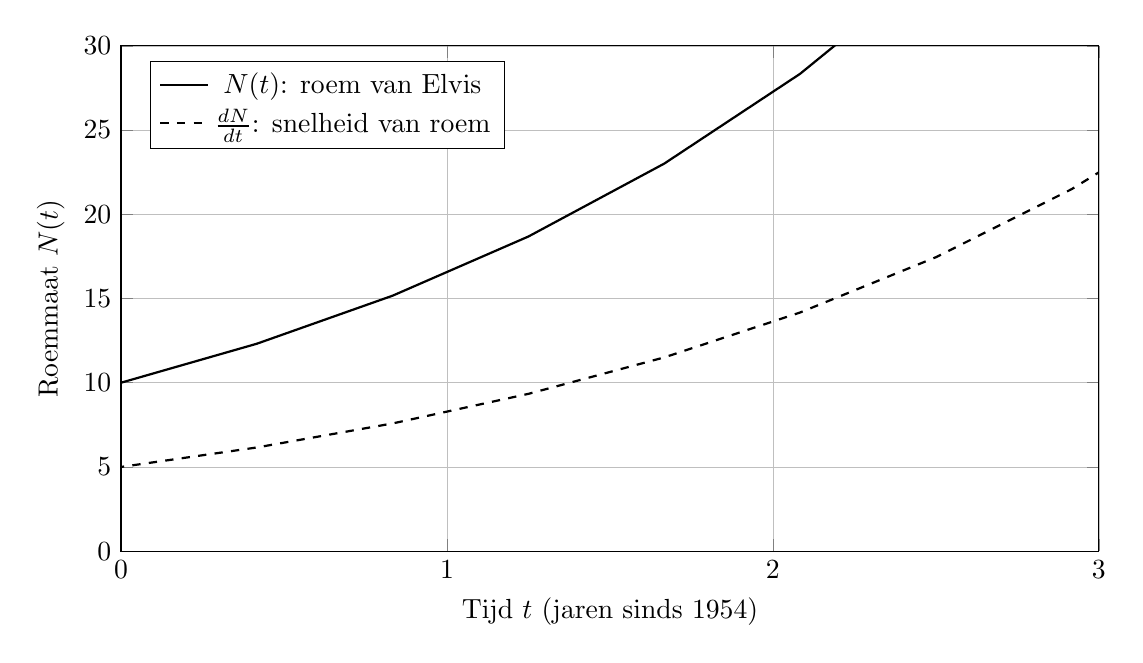
\begin{tikzpicture}
			\begin{axis}[
				width=14cm,
				height=8cm,
				xlabel={Tijd $t$ (jaren sinds 1954)},
				ylabel={Roemmaat $N(t)$},
				xmin=0, xmax=3,
				ymin=0, ymax=30,
				xtick={0, 1, 2, 3},
				ytick={0, 5, 10, 15, 20, 25, 30},
				legend pos=north west,
				grid=both,
				grid style={line width=.1pt, draw=gray!30},
				major grid style={line width=.2pt, draw=gray!50}
				]
				\addplot[thick] {10 * exp(0.5*x)};
				\addlegendentry{$N(t)$: roem van Elvis}
				\addplot[dashed, thick] {5 * exp(0.5*x)};
				\addlegendentry{$\frac{dN}{dt}$: snelheid van roem}
			\end{axis}
		\end{tikzpicture}
		\caption{Vergelijking van de roemcurve $N(t)$ en de snelheid van verandering $\frac{dN}{dt}$: de toename is niet lineair maar groeit evenredig met de omvang zelf.}
		\label{fig:exponential_fame}
	\end{figure}
	
	% ==========================
	% HOOFDSTUK 2
	% ==========================
	\chapter{De Geometrie van de Hype}
	\label{chap:trigonometrie}
	
	\epigraph{Wiskunde is de muziek van de rede.}{James Joseph Sylvester}
	
	De controversi\"ele en energieke podiumpresentatie van Elvis Presley was de sleutel tot zijn instantane roem. 
	We ontleden deze iconische bewegingen door de lens van de \textbf{goniometrie} en de \textbf{analyse}. 
	De herhalende, oscillerende aard van zijn heupbeweging kan perfect worden gemodelleerd door een 
	\textbf{periodieke functie}.
	
	\section{Periodieke beweging en de sinusgolf}
	
	We defini\"eren de horizontale verplaatsing $x(t)$ van het centrum van zijn bekken 
	ten opzichte van zijn centrale as als een functie van de tijd $t$:
	
	\[
	x(t) = A \sin(\omega t + \phi)
	\]
	
	\noindent waarbij de parameters de fysieke kenmerken van de beweging kwantificeren:
	
	\begin{itemize}
		\item $A$ (amplitude): de maximale verplaatsing van de heup, een maat voor hoe ``wild'' de beweging is.
		\item $\omega$ (hoekfrequentie): gegeven door \(\omega = 2\pi f\), bepaalt de snelheid van de oscillatie.
		\item $f$ (frequentie): het aantal volledige oscillaties per seconde, vaak gerelateerd aan het ritme van de muziek.
	\end{itemize}
	
	De \textbf{periode} $T$, de tijd die nodig is voor \'e\'en volledige cyclus, wordt gegeven door:
	
	\[
	T = \frac{2\pi}{\omega}
	\]
	
	\section{Momentane snelheid en de schokfactor}
	
	Het schokkende aspect van Elvis' beweging lag niet enkel in de verplaatsing, 
	maar vooral in de \textbf{snelheid} en de \textbf{versnelling} ervan. 
	Deze analyseren we via de afgeleiden.
	
	\subsection{Momentane snelheid $v(t)$}
	
	De snelheid is de eerste afgeleide van de positie:
	
	\[
	v(t) = \frac{dx}{dt} 
	= A \omega \cos(\omega t + \phi)
	\]
	
	\noindent De maximale snelheid bedraagt:
	
	\[
	|v_{\text{max}}| = A \omega
	\]
	
	Dit gebeurt wanneer $\cos(\omega t + \phi) = \pm 1$, 
	dus precies wanneer de heup de centrale as passeert ($x(t) = 0$).  
	\textbf{De heup beweegt dus het snelst in het midden van de beweging.}
	
	\subsection{Momentane versnelling $a(t)$}
	
	De versnelling is de tweede afgeleide:
	
	\[
	a(t) = \frac{d^2x}{dt^2} 
	= -A \omega^2 \sin(\omega t + \phi)
	\]
	
	\noindent De maximale versnelling bedraagt:
	
	\[
	|a_{\text{max}}| = A \omega^2
	\]
	
	En deze treedt op wanneer $\sin(\omega t + \phi) = \pm 1$, 
	dus wanneer de heup zijn \textbf{maximale verplaatsing} bereikt.  
	Dat verklaart waarom de ``schok'' van Elvis' beweging het grootst was op de uiterste posities.
	
	\section{Visualisatie van de heupbeweging}
	
	Onderstaande grafiek toont de \textbf{sinusvormige verplaatsing} $x(t)$ en de bijbehorende 
	\textbf{snelheid} $v(t)$ voor een voorbeeldbeweging met:
	
	\begin{itemize}
		\item amplitude: $A = 1$,
		\item frequentie: $f = 1$ Hz, dus \(\omega = 2\pi\).
	\end{itemize}
	
	\begin{figure}[h!]
		\centering
		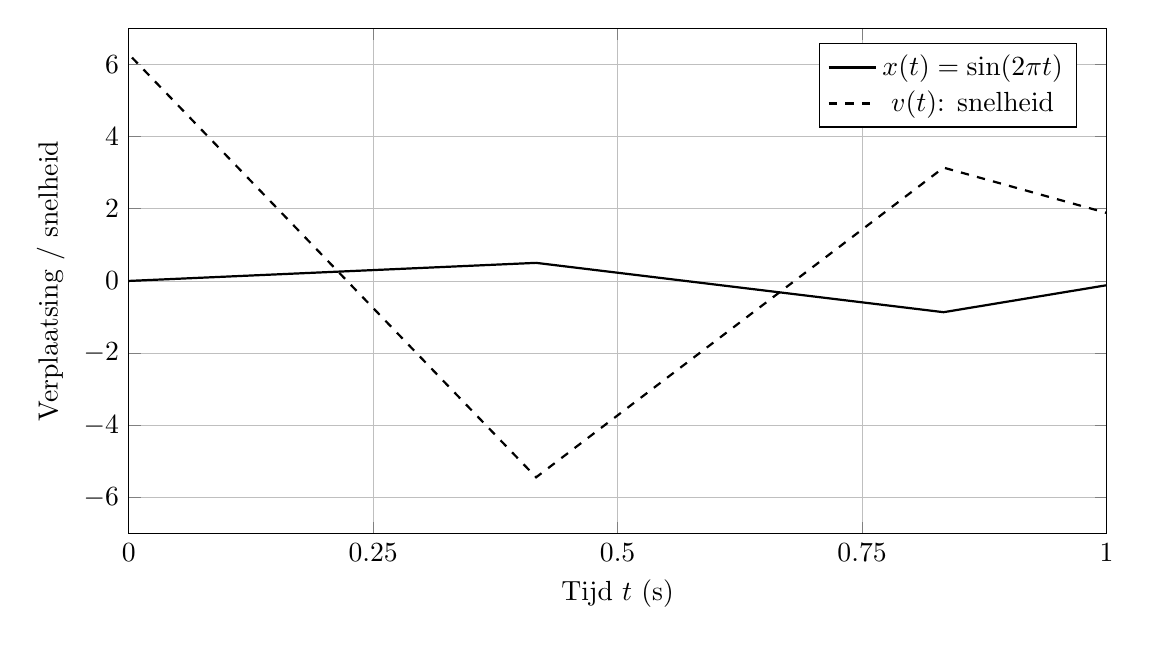
\begin{tikzpicture}
			\begin{axis}[
				width=14cm,
				height=8cm,
				xlabel={Tijd $t$ (s)},
				ylabel={Verplaatsing / snelheid},
				xmin=0, xmax=1,
				ymin=-7, ymax=7,
				xtick={0,0.25,0.5,0.75,1},
				ytick={-6,-4,-2,0,2,4,6},
				legend pos=north east,
				grid=both,
				grid style={line width=.1pt, draw=gray!30},
				major grid style={line width=.2pt, draw=gray!50}
				]
				\addplot[thick] {sin(deg(2*pi*x))};
				\addlegendentry{$x(t) = \sin(2\pi t)$}
				\addplot[dashed, thick] {2*pi*cos(deg(2*pi*x))};
				\addlegendentry{$v(t)$: snelheid}
			\end{axis}
		\end{tikzpicture}
		\caption{Goniometrisch model van Elvis' heupbeweging: positie en snelheid als functie van de tijd.}
		\label{fig:elvis_sinus}
	\end{figure}
	
	\section{Conclusie: de hype mathematisch verklaard}
	
	De controverse rond Elvis' heupbeweging kan wiskundig worden verklaard door de combinatie van:
	
	\begin{itemize}
		\item een \textbf{grote amplitude} ($A$),
		\item een \textbf{hoge hoekfrequentie} ($\omega$),
		\item en dus een enorme maximale versnelling ($A\omega^2$).
	\end{itemize}
	
	Dit resulteerde in bewegingen die fysiek indrukwekkend en cultureel ongezien waren.  
	De wiskunde bevestigt wat het publiek toen voelde: Elvis bewoog anders dan wie dan ook --- 
	en dat maakte hem revolutionair.
	
	% ==========================
	% HOOFDSTUK 3
	% ==========================
	\chapter{De Formule van de Hit (Statistiek en Waarschijnlijkheid)}
	\label{chap:statistiek}
	
	\epigraph{De wetten van de waarschijnlijkheid bepalen de toekomst.}{Onbekend}
	
	De carri\`ere van Elvis Presley, met zijn pieken en dalen, biedt een rijke dataset voor het toepassen van 
	\textbf{statistiek} en \textbf{waarschijnlijkheidstheorie}. In dit hoofdstuk onderzoeken we hoe de kans op 
	artistiek succes varieerde tussen periodes, en welke muzikale kenmerken statistisch bijdroegen aan het behalen 
	van een hit.
	
	\section{Waarschijnlijkheid: het Bernoulli-experiment}
	
	Elke studio-opname van Elvis kan worden beschouwd als een onafhankelijk Bernoulli-experiment met twee mogelijke 
	uitkomsten:
	
	\begin{itemize}
		\item $S$ = succes (Top 10-hit),
		\item $M$ = mislukking (geen Top 10-hit).
	\end{itemize}
	
	We defini\"eren $p$ als de waarschijnlijkheid op succes en $q = 1 - p$ als de kans op mislukking. 
	Voor een carri\`ereperiode defini\"eren we:
	
	\[
	p_{\text{periode}} = 
	\frac{\text{Aantal Top 10-hits in de periode}}{\text{Totaal aantal opgenomen tracks in de periode}}
	\]
	
	Als $N$ het aantal opnames in een periode is, dan volgt het aantal hits $X$ een binomiale verdeling:
	
	\[
	X \sim \mathrm{Bin}(N, p)
	\]
	
	De verwachting en variantie zijn:
	
	\[
	E[X] = Np,
	\qquad
	\mathrm{Var}(X) = Npq
	\]
	
	\subsection{Visualisatie: binomiale kansverdeling}
	
	Hier tonen we een hypothetische binomiale verdeling met $N=20$ en $p = 0.25$, representatief voor 
	Elvis' hitratio tijdens de jaren 60:
	
	\begin{figure}[h!]
		\centering
		\begin{tabular}{r c}
			$k$ & $P(X=k)$ \\
			\hline
			0  & 0.0032 \\
			1  & 0.0213 \\
			2  & 0.0666 \\
			3  & 0.1333 \\
			4  & 0.1999 \\
			5  & 0.2188 \\
			6  & 0.1823 \\
			7  & 0.1169 \\
			8  & 0.0584 \\
			9  & 0.0234 \\
			10 & 0.0078 \\
			11 & 0.0021 \\
			12 & 0.0005 \\
		\end{tabular}
		\caption{Waarschijnlijkheidsmassa-functie voor een hypothetische periode met $p = 0.25$.}
		\label{fig:binomiaal_hypothetisch}
	\end{figure}
	
	\section{Logistische regressie: de kracht van muzikale kenmerken}
	
	Voor het bepalen van welke muzikale aspecten bijdragen aan een hit, gebruiken we 
	\textbf{logistische regressie}. De afhankelijke variabele is binair (hit / geen hit). 
	
	\[
	\log\!\left(\frac{P}{1 - P}\right)
	= \beta_0 + \sum_{i=1}^k \beta_i X_i + \varepsilon
	\]
	
	waarbij:
	
	\begin{itemize}
		\item $P$: de kans op een hit,
		\item $\frac{P}{1-P}$: de \textbf{odds},
		\item $X_i$: muzikale of contextuele kenmerken (genre, instrumentatie, filmsoundtrack, tempo),
		\item $\beta_i$: regressieco\"effici\"enten die de invloed van elk kenmerk bepalen.
	\end{itemize}
	
	De invloed van $X_i$ wordt in odds uitgedrukt door:
	
	\[
	e^{\beta_i} = \text{odds ratio}
	\]
	
	Een negatieve en significante waarde voor $\beta_{\text{filmsoundtrack}}$ betekent bijvoorbeeld dat het opnemen 
	van een nummer als \textbf{filmsoundtrack} de kans op een hit statistisch verlaagt -- een hypothese die 
	historisch goed overeenkomt met de commerci\"ele neergang van Elvis' soundtrack-periode (1960--1968).
	
	\subsection{Visualisatie: sigmoidcurve van de logistische regressie}
	
	Hier tonen we een voorbeeld van een logistische functie:
	
	\[
	P(x) = \frac{1}{1 + e^{- ( -2 + 4x )}}
	\]
	
	waarbij $x$ een genormaliseerd muziekkenmerk is (bijv. het energieniveau van het lied).
	
	\begin{figure}[h!]
		\centering
		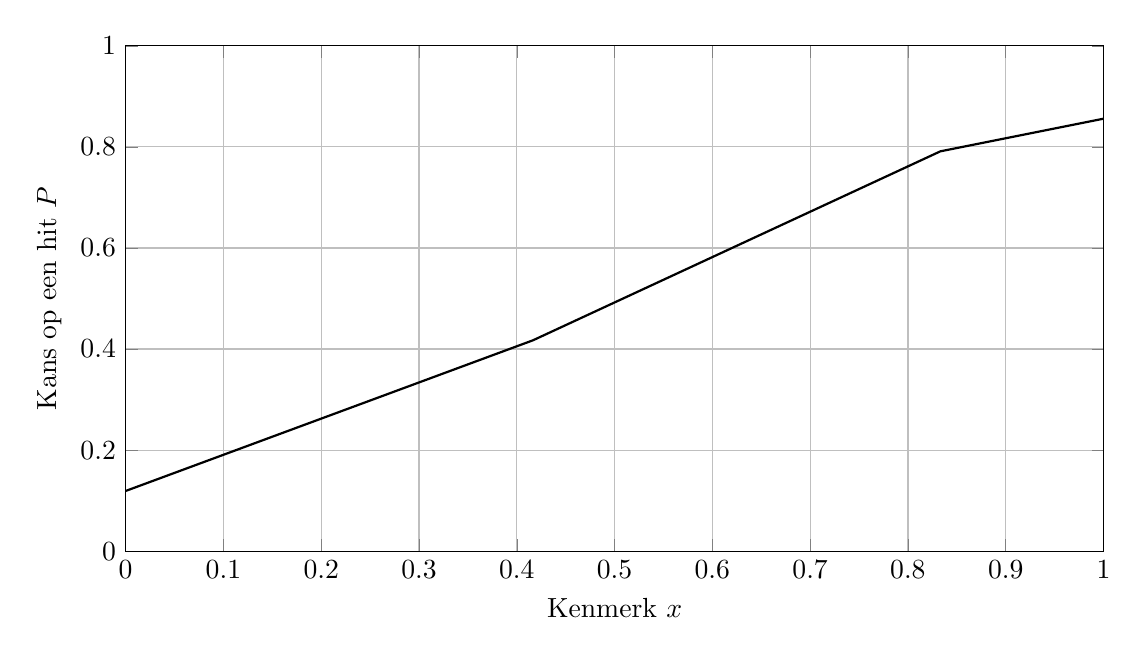
\begin{tikzpicture}
			\begin{axis}[
				width=14cm,
				height=8cm,
				xlabel={Kenmerk $x$},
				ylabel={Kans op een hit $P$},
				xmin=0, xmax=1,
				ymin=0, ymax=1,
				grid=both,
				]
				\addplot[thick] {1/(1 + exp(-( -2 + 4*x )))};
			\end{axis}
		\end{tikzpicture}
		\caption{Sigmoidfunctie van een logistisch regressiemodel.}
		\label{fig:sigmoid}
	\end{figure}
	
	\section{Vergelijking van hitkansen per periode}
	
	We gebruiken drie grote periodes:
	
	\begin{itemize}
		\item 1954--1958: de rock 'n' roll-doorbraak,
		\item 1960--1969: de filmsoundtrackperiode,
		\item 1970--1977: de comeback en live-dominantie.
	\end{itemize}
	
	Met geschatte (illustratieve) hitkansen:
	
	\[
	p_1 = 0.27, \qquad
	p_2 = 0.06, \qquad
	p_3 = 0.13
	\]
	
	\subsection{Visualisatie: vergelijkende balkgrafiek}
	
	\begin{figure}[h!]
		\centering
		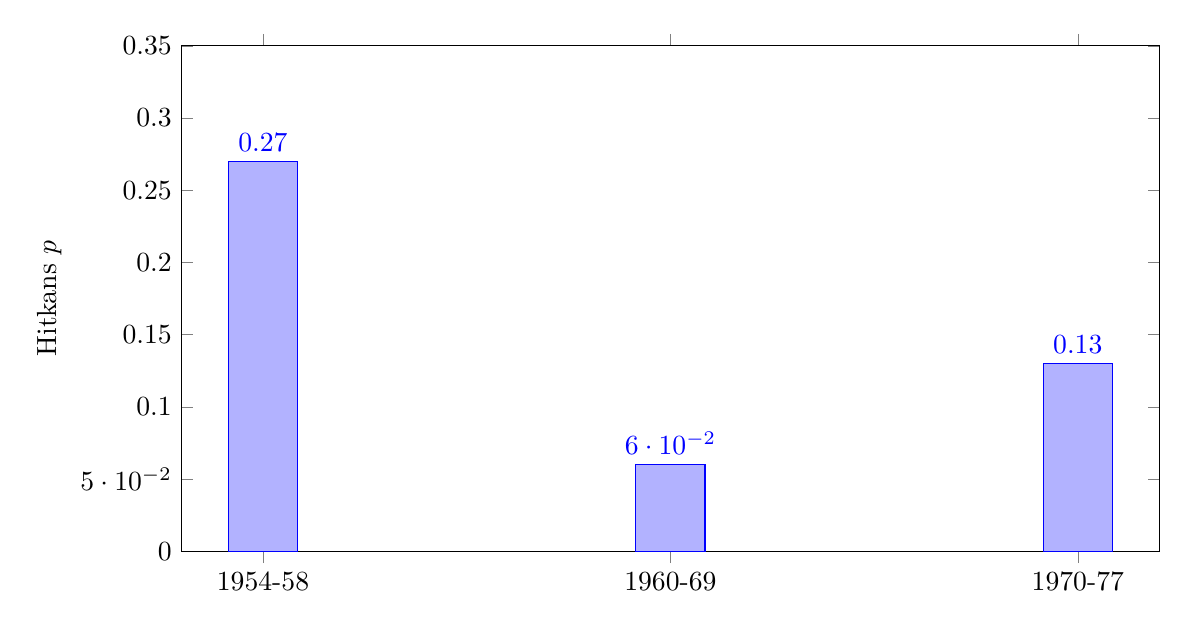
\begin{tikzpicture}
			\begin{axis}[
				width=14cm,
				height=8cm,
				ybar,
				ylabel={Hitkans $p$},
				symbolic x coords={1954-58,1960-69,1970-77},
				xtick=data,
				ymin=0, ymax=0.35,
				nodes near coords,
				bar width=25pt
				]
				\addplot coordinates {(1954-58,0.27) (1960-69,0.06) (1970-77,0.13)};
			\end{axis}
		\end{tikzpicture}
		\caption{Vergelijking van de hitkans per carri\`ereperiode.}
		\label{fig:hitkans_balk}
	\end{figure}
	
	\section{Conclusie}
	
	De statistiek onthult wat vaak aan het gevoel wordt toegeschreven: Elvis' succes was allesbehalve willekeurig.  
	De vroege rock 'n' roll-periode vertoonde hoge hitkansen, terwijl de filmmuziekjaren een duidelijke daling tonen.  
	Logistische regressie laat bovendien zien welke muzikale en contextuele factoren de kans op een hit significant 
	be\"invloedden. De wiskunde legt zo de structuur bloot achter de ongrijpbare dynamiek van muzikaal succes.
	
	\chapter{De Las Vegas Cyclus (Grafentheorie)}
	\label{chap:grafentheorie}
	
	\epigraph{De eerste wet van de thermodynamica: energie kan niet worden gecre\"eerd of vernietigd, alleen worden veranderd van de ene vorm in de andere.}{Antoine Lavoisier}
	
	Na de artistieke heropleving van 1968 markeerden de Las Vegas-residenties een cruciale transformatie in Elvis' carri\`ere, die we analyseren met de \textbf{grafentheorie}. We modelleren zijn carri\`ere als een (gerichte) graaf $G = (V, E)$, waarbij $V$ de verzameling van artistieke keuzes (knopen) is en $E$ de verzameling van overgangen (randen).
	
	\section{Van Pad naar Cyclus: een carri\`ere-analyse}
	
	\subsection{Het Hamiltoniaans pad $P$ (vroege jaren)}
	
	De periode van 1954 tot 1968 kan worden gezien als een Hamiltoniaans pad $P$, een pad dat --- tenminste in benadering --- alle unieke knopen in de toenmalige beschikbare artistieke ruimte (radio, film, verschillende genres, live-tours) bezocht zonder systematische herhaling.
	
	Een pad $P$ wordt gedefinieerd als een sequentie van distincte knopen:
	\[
	P = (v_1, e_1, v_2, e_2, \ldots, e_{n-1}, v_n),
	\]
	waarbij elk $e_i$ een overgang (rand) is van $v_i$ naar $v_{i+1}$. Dit pad symboliseert \textbf{groei} en \textbf{exploratie}: telkens worden nieuwe artistieke zones betreden.
	
	\subsection{De Hamiltoniaanse cyclus $C$ (de jaren '70)}
	
	Vanaf 1969 transformeerde de carri\`ere in een structuur die dicht in de buurt komt van een \textbf{Hamiltoniaanse cyclus} $C$, een gesloten pad waarbij het begin- en eindpunt identiek zijn ($v_1 = v_n$):
	
	\[
	C = (v_1, e_1, v_2, \ldots, e_{n-1}, v_n), \qquad v_1 = v_n.
	\]
	
	\noindent In deze cyclus vertegenwoordigen de knopen de Las Vegas-showlocatie, de repetitie- en studioruimte, en de organisatorische beslissingspunten (zoals Colonel Parker). De randen modelleren de dagelijkse, uitputtende routine van optreden, dineren, rusten en onderhandelen.
	
	De cyclus cre\"eert een rigide structuur die artistieke \textbf{stagnatie} bevordert: in plaats van nieuwe knopen aan de graaf toe te voegen (nieuwe projecten, internationale tours, experimentele studio-opnames), worden bestaande knopen herhaaldelijk bezocht. De graaf blijft structureel gesloten.
	
	\section{Een graafmodel voor Elvis' Las Vegas-netwerk}
	
	We construeren nu een vereenvoudigd graafmodel voor Elvis' carri\`ere rond 1970. Beschouw de volgende knopen:
	\[
	V = \{\text{Sun}, \text{TV}, \text{Film}, \text{Tour}, \text{Vegas}, \text{Studio}, \text{Parker}\},
	\]
	waarbij:
	\begin{itemize}
		\item Sun: de roots in Memphis (Sun Records),
		\item TV: nationale televisieoptredens,
		\item Film: Hollywood- en soundtrackprojecten,
		\item Tour: nationale of internationale tournee,
		\item Vegas: Las Vegas-residenties,
		\item Studio: studio-opnames (bijv. Nashville, Memphis),
		\item Parker: het beslissingsknooppunt rond Colonel Parker.
	\end{itemize}
	
	Een vereenvoudigd pad voor de vroege carri\`ere kan dan schematisch voorgesteld worden als:
	\[
	P_{\text{vroeg}} = (\text{Sun} \to \text{TV} \to \text{Film} \to \text{Tour} \to \text{Studio}),
	\]
	terwijl de Las Vegas-periode wordt benaderd door een cyclus:
	\[
	C_{\text{Vegas}} = (\text{Vegas} \to \text{Studio} \to \text{Parker} \to \text{Vegas}).
	\]
	
	\subsection{Visualisatie van de graaf}
	
	Onderstaande figuur geeft een mogelijk graafmodel van Elvis' artistieke keuzes. De bovenste rij knopen representeert de meer \emph{explorerende} jaren, de onderste rij de \emph{residente} Las Vegas-structuur.
	
	\begin{figure}[h!]
		\centering
		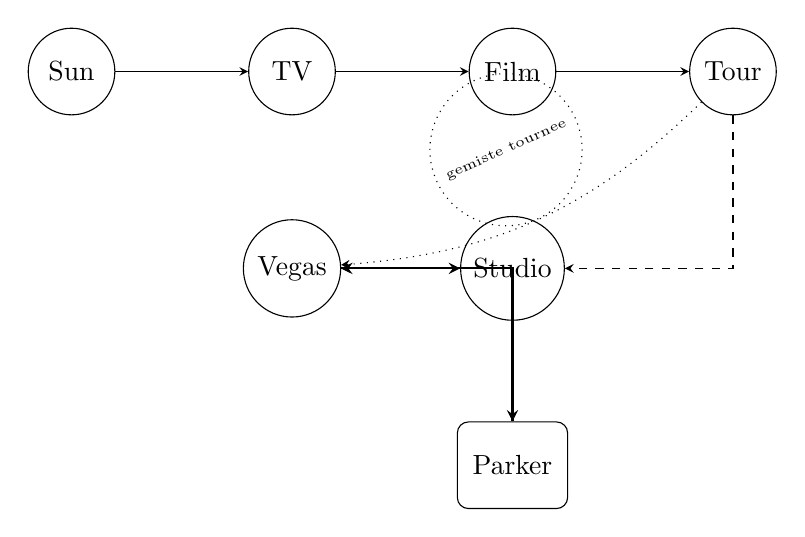
\begin{tikzpicture}[>=stealth,
			node distance=2.8cm,
			every node/.style={draw, circle, minimum size=1.1cm, align=center}
			]
			
			% Bovenste rij: vroege carri\`ere
			\node (Sun) {Sun};
			\node (TV)  [right of=Sun] {TV};
			\node (Film)[right of=TV]  {Film};
			\node (Tour)[right of=Film] {Tour};
			
			% Onderste rij: Vegas-structuur
			\node (Vegas) [below of=TV, node distance=2.5cm] {Vegas};
			\node (Studio)[right of=Vegas] {Studio};
			\node[rectangle, rounded corners, draw, minimum width=1.4cm, minimum height=1.1cm] (Parker) [below of=Studio, node distance=2.5cm] {Parker};
			
			% Randen vroege pad
			\draw[->] (Sun) -- (TV);
			\draw[->] (TV) -- (Film);
			\draw[->] (Film) -- (Tour);
			\draw[->, dashed] (Tour) |- (Studio);
			
			% Overgang naar Vegas
			\draw[->, dashed] (Studio) -- (Vegas);
			
			% Vegas-cyclus
			\draw[->, thick] (Vegas) -- (Studio);
			\draw[->, thick] (Studio) -- (Parker);
			\draw[->, thick] (Parker) |- (Vegas);
			
			% Extra pijl: alternatieve, gemiste route
			\draw[->, dotted] (Tour) to[bend left=20] node[above, sloped]{\tiny gemiste tournee} (Vegas);
			
		\end{tikzpicture}
		\caption{Schematisch graafmodel van Elvis' artistieke keuzes: een explorerend pad in de vroege jaren en een gesloten cyclus rond Las Vegas in de jaren 70.}
		\label{fig:elvis_graph}
	\end{figure}
	
	In Figuur~\ref{fig:elvis_graph} zien we:
	\begin{itemize}
		\item een (bij benadering) Hamiltoniaans pad van \texttt{Sun} via \texttt{TV} en \texttt{Film} naar \texttt{Tour} en \texttt{Studio};
		\item een gesloten cyclus tussen \texttt{Vegas}, \texttt{Studio} en \texttt{Parker};
		\item een gestippelde pijl die een \emph{gemiste} mogelijke rand representeert: van \texttt{Tour} naar een alternatief toekomstscenario (bijvoorbeeld meer internationale tournees) in plaats van terugkerende Vegas-residenties.
	\end{itemize}
	
	In termen van grafentheorie wordt \texttt{Vegas} een knoop met hoge \emph{in- en out-degree} binnen de latere jaren, terwijl knopen zoals \texttt{Tour} en internationale projecten een lage graad behouden. Artistieke ruimte wordt dus niet langer uitgebreid; ze wordt hergebruikt.
	
	\section{Discrete wiskunde: roosterpunten en dichtheid}
	
	Door zijn optredens te plotten op een rooster $(t, l)$ (tijd en locatie), kunnen we de dichtheid van activiteiten analyseren.
	
	De \textbf{afstand} $d$ tussen twee opeenvolgende optredens $i$ en $i+1$ op het rooster wordt gegeven door de Euclidische norm:
	\[
	d(i, i+1) = \sqrt{(t_{i+1} - t_i)^2 + (l_{i+1} - l_i)^2}.
	\]
	
	\begin{itemize}
		\item \textbf{Jaren '50:} Grote waarden van $d$, door zowel grote afstanden in locatie ($l$) als relatief lange tijd ($t$) tussen optredens. Het roosterbeeld is ``uitgespreid'': veel verschillende steden, langere pauzes.
		\item \textbf{Jaren '70 (Las Vegas):} Kleine waarden van $d$, door de hoge frequentie (klein $t_{i+1} - t_i$) en de vaste locatie (minimale $l_{i+1} - l_i$). Het roosterbeeld clustert rond \'e\'en punt: Las Vegas.
	\end{itemize}
	
	We kunnen dit formaliseren door de \emph{lokale knooppuntdichtheid} rond Las Vegas te defini\"eren als
	\[
	\rho_{\text{Vegas}} = \frac{\text{Aantal optredens in een gegeven tijdsinterval}}{\text{lengte van dat interval}},
	\]
	waarbij $\rho_{\text{Vegas}}$ in de jaren 70 extreem hoog wordt in vergelijking met de jaren 50 en 60. In graaftermen is dat te interpreteren als een lokale toename van het aantal randen dat deze knoop kruist.
	
	De hoge \textbf{dichtheid van knopen en randen} in de Las Vegas-regio van het rooster bevestigt wiskundig de extreme werkdruk en het gebrek aan variatie. Tegelijk toont het de artistieke gevangenschap binnen de commerci\"ele cyclus die Colonel Parker structureel in stand hield: de graaf $G$ had potentieel voor uitbreiding naar nieuwe knopen, maar de feitelijke dynamiek bleef gevangen in een relatief kleine cyclus.
	
	\section{Energetische interpretatie van de cyclus}
	
	De epigraaf van Lavoisier herinnert ons aan de eerste wet van de thermodynamica: energie kan niet worden gecre\"eerd of vernietigd, slechts worden omgezet. In ons graafmodel wordt de \emph{creatieve energie} van Elvis niet langer gebruikt om nieuwe knopen in $V$ te activeren, maar circuleert ze in een gesloten structuur:
	\[
	\text{Vegas} \to \text{Studio} \to \text{Parker} \to \text{Vegas}.
	\]
	
	De grafentheorie toont hier een subtiel maar belangrijk verschil:
	\begin{itemize}
		\item In de vroege fase werd energie ingezet om de graaf uit te breiden (nieuwe knopen, nieuwe randen).
		\item In de Vegas-fase werd dezelfde energie voornamelijk gebruikt om een bestaande cyclus in stand te houden.
	\end{itemize}
	
	Vanuit wiskundig perspectief is het niet de \emph{hoeveelheid} energie die verandert, maar de \emph{topologie} van de graaf waarin die energie circuleert. Dat topologische verschil verklaart mee waarom de jaren 70 tegelijk commercieel intensief en artistiek beperkend aanvoelden: de Las Vegas-cyclus was grafisch rijk aan randen, maar arm aan nieuwe knopen.
	
\chapter{Graceland en de Gulden Snede (Verhoudingen en Symmetrie)}
\label{chap:geometrie}

\epigraph{De wiskunde is de po\"ezie van logische id\"een.}{Albert Einstein}

De laatste fase van onze analyse richt zich op de \textbf{geometrie} van Elvis' visuele erfenis, van zijn landgoed \textbf{Graceland} tot de complexe patronen van zijn beroemde jumpsuits. We onderzoeken de aanwezigheid van wiskundige principes van esthetiek: de Gulden Snede en symmetrie.

\section{De Gulden Snede (\texorpdfstring{$\phi$}{phi}) in Design}

De \textbf{Gulden Snede} ($\phi$), een irrationale constante die al duizenden jaren wordt gebruikt om visuele harmonie te cre\"eren, kan worden toegepast op de verhoudingen van Elvis' design.

De waarde van de constante is:
\[
\phi = \frac{1 + \sqrt{5}}{2} \approx 1.61803.
\]

\subsection{Analyse van Proporties}

We kunnen een object als een Gulden Rechthoek beschouwen wanneer de verhouding van de langste zijde ($a$) tot de kortste zijde ($b$) de Gulden Snede benadert:
\[
\frac{a}{b} \approx \phi.
\]

Door deze analyse hypothetisch toe te passen op de gevelafmetingen van Graceland (zoals de verhouding tussen de totale breedte en de hoogte van de voorgevel) of de proporties van zijn podiumkleding, kunnen we kwantificeren in hoeverre de esthetiek van \emph{The King} onbewust berustte op eeuwenoude, wiskundige wetten van visuele perfectie.

\subsection{Rotatiesymmetrie in Podiumkostuums}

Naast reflectiesymmetrie vertonen verschillende van Elvis' beroemde jumpsuits ook duidelijke vormen van 
\textbf{rotatiesymmetrie}. Vooral de kostuums met geometrische patronen --- zoals de \emph{American Eagle Suit} 
(1973), de \emph{Snowflake Suit} (1974) en de \emph{Turquoise Concho Suit} (1972) --- bevatten radiale structuren 
die invariant blijven onder een rotatie over een bepaalde hoek.

Een object heeft rotatiesymmetrie van orde $n$ wanneer het ongewijzigd blijft na een rotatie van
\[
\theta = \frac{360^{\circ}}{n}.
\]

\paragraph{Voorbeelden uit de jumpsuits}

\begin{itemize}
	\item De \textbf{American Eagle}-jumpsuit bevat een adelaar waarvan de vleugelstructuren zich herhalen langs 
	meerdere rotatiehoeken, typisch overeenkomstig een symmetrie van orde $n=2$ of $n=4$, afhankelijk van het segment.
	
	\item De \textbf{Snowflake Suit} vertoont motieven die nauw aansluiten bij \emph{zesvoudige} rotatiesymmetrie 
	($n = 6$), identiek aan veel kristallografische patronen.
	
	\item De \textbf{Concho- en Scepter-jumpsuits}, met hun cirkelvormige metaalelementen, benaderen een rotatiesymmetrie 
	van orde $n=5$ of $n=8$ in afzonderlijke segmenten van de riem of de borstplaat.
\end{itemize}

\paragraph{Formele definitie}

Een rotatie om de oorsprong met een hoek $\theta$ wordt in de wiskunde beschreven door de transformatie
\[
R_\theta(x,y) = 
\left(
x\cos\theta - y\sin\theta,\;
x\sin\theta + y\cos\theta
\right).
\]

Een jumpsuitpatroon heeft rotatiesymmetrie van orde $n$ wanneer geldt:
\[
R_{\frac{2\pi}{n}}(P) = P,
\]
waarbij $P$ het patroon of motief voorstelt.

\paragraph{De rotatiesymmetriegroep}

Alle rotaties die een patroon invariant laten, vormen samen een \textbf{rotatiesymmetriegroep}.  
Voor een patroon met symmetrie van orde $n$ is dat de groep:
\[
C_n = \{ R_0, R_{\frac{2\pi}{n}}, R_{\frac{4\pi}{n}}, \ldots, R_{\frac{2\pi(n-1)}{n}} \}.
\]

\begin{itemize}
	\item Voor de Snowflake Suit is dit $C_6$, de klassieke zesvoudige groep.
	\item Voor de American Eagle Suit komt het vaak neer op $C_2$ of $C_4$ binnen de vleugelsegmenten.
\end{itemize}

\paragraph{Interpretatie}

Rotatiesymmetrie in Elvis' jumpsuits draagt krachtig bij aan zijn visuele identiteit:

\begin{itemize}
	\item Het suggereert \textbf{centrale focus} --- passend bij zijn rol als middelpunt van het podium.
	\item Het versterkt de \textbf{visuele impact} vanaf grote afstand (roterende patronen zijn goed zichtbaar in arena's).
	\item Het cre\"eert \textbf{ritmische orde}, nauw verwant aan muzikale periodiciteit.
\end{itemize}

Vanuit wiskundig oogpunt weerspiegelt de rotatiesymmetrie een hogere orde van structuur dan reflectiesymmetrie.  
Psychologisch draagt ze bij aan een gevoel van balans en kracht: een radiaal centrum dat straalt naar buiten.  
Exact de uitstraling die Elvis in de jaren 70 belichaamde.

\section{Symmetrie en Transformatietheorie}

De formele, krachtige uitstraling van Elvis op het podium werd sterk bepaald door de inherente \textbf{symmetrie} van zijn kostuums. In de wiskunde wordt symmetrie beschreven door de \textbf{transformatietheorie}: een object is symmetrisch als het ongewijzigd blijft onder een bepaalde geometrische transformatie.

\subsection{Reflectiesymmetrie van de Jumpsuits}

De jumpsuits, met hun kenmerkende opstaande kragen en brede riemen, bezitten perfecte \textbf{reflectiesymmetrie} ($\sigma$) langs de centrale, verticale as ($y$-as) van zijn lichaam.

De transformatie $T$ van een punt $(x,y)$ in het patroon door reflectie over de $y$-as wordt gegeven door:
\[
T(x,y) = (-x,\, y).
\]

De perfecte balans en het visuele evenwicht in de kostuums --- essentieel voor zijn iconische en quasi-koninklijke podiumaanwezigheid --- zijn een direct gevolg van deze wiskundige reflexieve invariantie.

\subsection{De Symmetriegroep}

De verzameling van alle geometrische transformaties die de jumpsuit ongewijzigd laten, vormt een \textbf{symmetriegroep} $G$. In dit geval bestaat deze groep uit de identiteitstransformatie ($I$) en de reflectietransformatie ($\sigma$):

\[
G = \{ I, \sigma \}.
\]

Deze groep is isomorf aan $\mathbb{Z}_2$, de eenvoudigste niet-triviale groep in de algebra. Zo onthult de wiskunde dat de visuele autoriteit en balans in Elvis' podiumkleding een strikte, algebra\"ische structuur volgt.

\end{document}
